\chapter{System}\label{ch:system}

This chapter contains more information about the structure of the project. Figure \ref{fig:Deployment_Model} shows all devices and their communication interfaces of the whole system. There are three subdivisions:

\begin{itemize}
	\item Charging Station
	\item Electric Vehicle
	\item RTK Base Station
\end{itemize}

The vehicle and the charging station communicate with the RSU and the OBU over an ITS-G5 link. In order to use the application layer of the MK5 units, an expensive SDK would be needed. Because of this, the application is running on a Raspberry Pi. The MK5 units run an application, which offers an UDP interface for sending and receiving BTP packets. This is explained in section \ref{sec:BTP_over_UDP}.

The RTK base station sends the RTCM correction data over an internet connection to the vehicle. It can calculate its position much more precisely with this information.

\begin{figure}[htb]
	\centering
	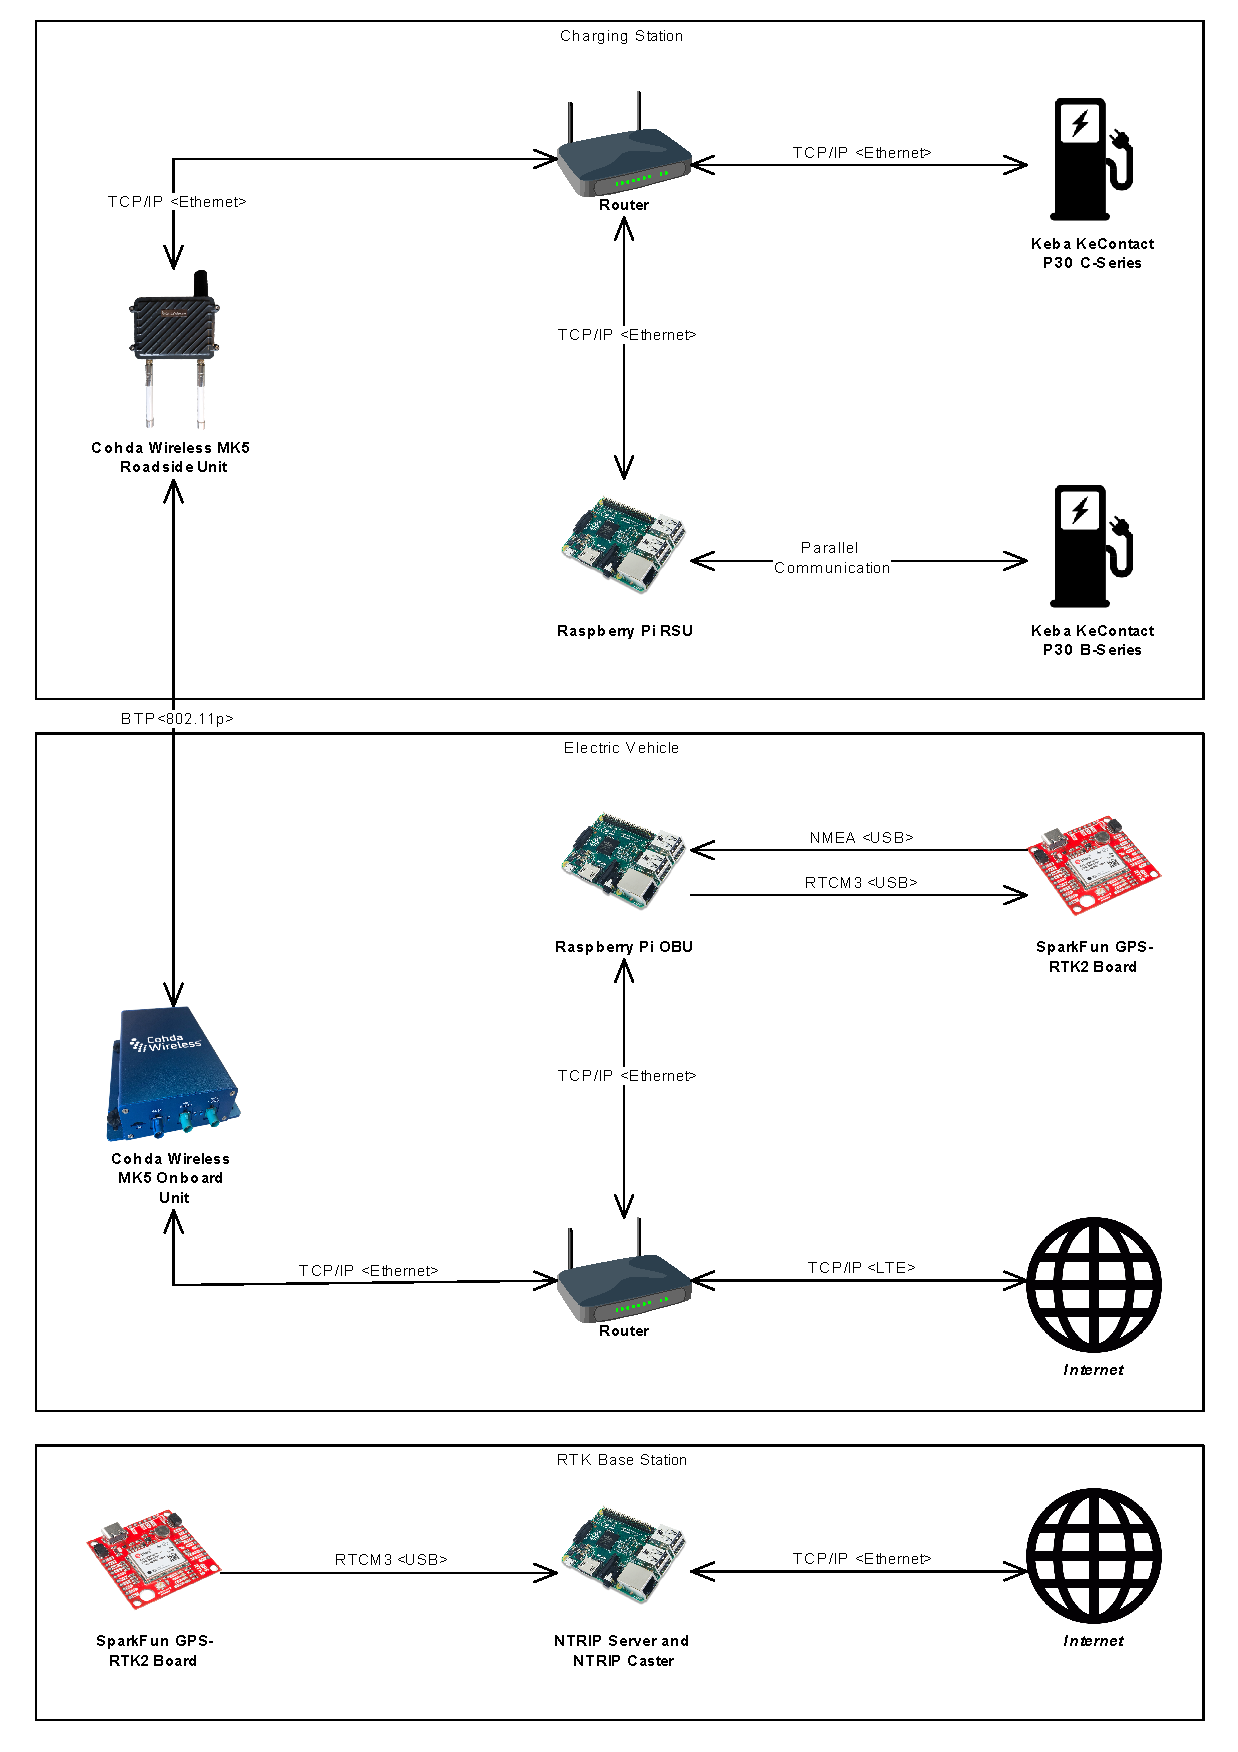
\includegraphics[width=1\textwidth]{images/model}
	\caption{Deployment Diagram}
	\label{fig:Deployment_Model}
\end{figure}

\clearpage
\pagebreak


\section{Charging Station}

The charging station consists of two charging devices, a Raspberry Pi, a MK5 roadside unit and an external router, which manages the communication in the subsystem. The Raspberry Pi runs the firmware that controls the whole charging station. Depending on which parking lot the electric vehicle is positioned, one of the charging devices gets unlocked. All components of the charging station communicate with TCP/IP, excluding the b-series charging device.

\subsection{Control of the Charging Device}

The b-series, which is installed on the campus, can be unlocked with a simple relay switch. Therefore a module with a relay was needed. The GPIOs of the Raspberry Pi are not able to supply the relay directly. For this reason a transistor driver was implemented. The charging station has an output, which registers if the car is plugged in or not. With this information, the system knows if a charging session is requested or whether it is finished. The charging port will only be released if the car parks on the right parking lot. The driver has 1\;min to plug in the vehicle after it is parked.

Micaro provided a second charging station c-series for test purposes. It is able to unlock its charging port over Ethernet with UDP. This solution requires only an Ethernet cable and is fairly save. Additionally the charging station can communicate with the Raspberry Pi. Therefore the Raspberry Pi knows in what state the charging station is and it can set parameters (e.g. the maximum output current).
\newpage
\section{Electric Vehicle}

The electric vehicle is equipped with a Raspberry Pi, an MK5 onboard unit, a GNSS module and a router. Same as the charging station, the software runs on the Raspberry Pi. With a GNSS receiver and the correction data received over TCP, the vehicle can determine its position. The GNSS antenna is mounted in the roof box on the vehicle as seen in figure \ref{fig:AntennaMount}.

\begin{figure}[htb]
	\centering
	\includegraphics[width=0.7\textwidth]{images/AntennaMount}
	\caption{GNSS Antenna mounted on the Wireless Research Vehicle}
	\label{fig:AntennaMount}
\end{figure}


The rover is connected with the Raspberry Pi, which sends RTCM messages to the rover and receives NMEA data to get the position of the vehicle. With this housing illustrated in figure \ref{fig:RTKRover}, the RTCM data can be sent to the rover over USB and the second UART port. The USB connection is not able to transmit all NMEA, UBX and RTCM data with a refresh rate of 10\;Hz. However, with 5\;Hz it worked without any data loss and this refresh rate is high enough to fulfill the task.

\begin{figure}[htb]
	\centering
	\includegraphics[width=0.7\textwidth]{images/RTK-Rover}
	\caption{RTK Rover installed in the Vehicle}
	\label{fig:RTKRover}
\end{figure}

\newpage

\section{RTK Base Station} \label{sec:rtkBase}

The localization built in the Cohda Wireless system was not precise enough to detect that the vehicle is on the parking lot. The solution to this problem was a differential GNSS module which supports real time kinematic (RTK). \cite{WsCommScript}

The base station in figure \ref{fig:BaseStation} consists of a SparkFun board ZED-F9P and a Raspberry Pi 3. At the university, there is a dual band GNSS antenna installed, which is suitable for the base station. A Bias-Tee supplies this antenna with power and separates the RF signal to the u-blox module. This module calculates the correction data and sends it to a connected Raspberry Pi, which runs a stream-to-stream server. It represents an NTRIP server as seen in figure \ref{fig:NTRIP_model}. The NTRIP stream is built with RTKLIB, which is an open source program package for GNSS positioning. \cite{RTKLIB}

The base station is configured with u-center. This is a free GNSS evaluation software by u-blox to log data and configure their modules. The mode has to be set to base station and an accuracy limit has to be defined. The minimum accuracy it reaches is 5\;cm. If the parameter is set lower, the base station tries to get this more accurate position without any success \cite{ZED-F9P-IntegrationManual}.
After the configuration the board launches in 'Survey In' mode and tries to determine its position with the given accuracy. This takes a few hours when done from a cold start or a few minutes from a hot start. After a successful startup, it sends RTCM messages to the NTRIP server. \cite{NTRIP_RPi}

\begin{figure}[htb]
	\centering
	\includegraphics[width=0.5\textwidth]{images/Base_station}
	\caption{RTK Base Station}
	\label{fig:BaseStation}
\end{figure}
\newpage
\section{Communication}\label{sec:BTP_over_UDP}

All three subsystems communicate with each other. The correction data of the base station is sent to the Raspberry Pi in the vehicle over the internet connection. Additionally, both Raspberry Pis communicate via the V2X channel. 

\subsection{ETSI ETSA}

Cohda Wireless did not share the interfaces for GNSS and 802.11p without buying the Software Developer Kit. Therefore both MK5s only run a given program, the ETSA, which is provided by Cohda Wireless. It is the ETSI network library linked with a wrapper as a standalone program. It uses the advantages of the 802.11p standard for example low latency. This application offers an UDP interface for sending and receiving BTP packets (section \ref{sec:BTP}). External computers - in this case the Raspberry Pis - have to create and interpret these packets. This is described in section \ref{sec:BTPHeader}. The Cohda Wireless hardware only implements a V2X interface as demanded by the task. \cite{CohdaWirelessETSA}

The payload transmitted over the MK5s is encrypted with the Fernet function in Python. It is built on top of a number of standard cryptographic primitives and ideal for encrypting small amount of data, for example short messages. Fernet guarantees that a message encrypted using it can not be manipulated or read without a key, in other words it is implemented as a symmetric authentication cryptography. \cite{Fernet}

\subsection{BTP Header}\label{sec:BTPHeader}

To send data, the packet has to be built as seen in appendix \ref{app:BTPHeaderIndicationRequest}. The header contains information how the packets has to be sent. The packets can be sent in broadcast or unicast. If sent in broadcast, the header contains information about how far the packets have to be sent. In unicast instead of a distance there is an address to show to whom the message was directed.
For this project, the ITSGnSecurity does not work, because with this option enabled, the ItsGnLocalAddr changes over time. For broadcast messages, the BTP type B was used (non-interactive). For unicast messages, the interactive type A was chosen. The GoeNetworking protocol adapts the system of well-known ports from the internet protocol. These ports are reserved for a certain use. If an entity has no well-known port, the used port must be between 3000 and 65536. For this application port 44203 was used.

Table \ref{tab:btp_header} shows how the BTP headers are built in this thesis. \cite{CohdaWirelessETSA}



\begin{table}
\begin{tabular}{|l|c|l|}
	\hline
	\hline
	BTP Type & 2 & Type A: interactive (Unicast) \\
	& 1 & Type B: non-interactive (Broadcast) \\ \hline
	GN Packet Transport & 2  & Unicast  \\
	& 7 &  Broadcast \\ \hline
	GN Traffic Class & 1 & default priority  \\ \hline
	GN Max Pkt Lifetime & 0 & 0 = use parameter from configuration file  \\ \hline
	BTP Destination Port & AC,AB & port 44203  \\ \hline
	BTP Dest Port Info & 1,1 & encrypted  \\ 
	& 0,0 & not encrypted  \\ \hline
	GN Destination & 0,0 & \textit{no Address needed in broadcast}  \\ 
	& ItsGnLocalAddr,0 & GeoNetworkingAddress  \\ \hline
	GN Comms Profile & 0 & Profile G5 (\textit{others are not supported yet})  \\ \hline
	GN Repeat Interval & 0 & \textit{not supported yet}  \\ \hline
	GN Security & 0 & \textit{all security bytes set to 0}  \\ \hline
	Data Length & \#,\# & length of payload  \\ \hline
	Data[...]  & payload & messages  \\ \hline
	\hline
\end{tabular}
\caption{BTP Header as it is built for this project.}
\label{tab:btp_header}
\end{table}

\clearpage
\newpage

\section{Procedure}

The system was developed to work on the university campus. The procedure is built, in a way where no action by the driver is required.

%connection
The RSU sends BTP messages as long as there are empty charging ports, to show their availability. This message contains the address of the RSU to build an unicast connection, information about the location of the charging station and how many ports are available. The initial task of the OBU is to look for a charging station by receiving their BTP-packets. If both units get close to each other, the OBU receives the message from the RSU, which contains information about the charging station. With this data, the OBU can build an unicast to the RSU. Then both parties wait until the vehicle drives on to the parking area. This is necessary, because there has to be a stable connection between both units, to make sure the authentication can be done without packet loss.

%authenticaton
The vehicle sends its 'vehicle ID' to the charging station. The ID is checked by the Raspberry Pi, to determine whether the vehicle has the permission to charge at the charging station. If this is the case, the charging station grants permission to charge to the vehicle.

%parking
Subsequently, the driver has 2\;min to park his vehicle on any parking lot. After that, the vehicle sends the charging station the number of its selected parking lot. The charging station will then release the specific charging port. If the driver does not need to charge and parks the vehicle somewhere else nearby, both parties go back to their initial state.

%charging process and complete
The vehicle can be plugged in and the charging process begins. When the vehicle is charged or the process gets interrupted by a user, the RSU locks the port and offers it to other vehicles by broadcast message. The vehicle waits until it leaves the charging area, to change to its initial state, because otherwise the authentication process starts again, right after the Raspberry Pi and OBU have started up.

\begin{figure}[htb]
	\centering
	\includegraphics[width=1\textwidth]{images/activity}
	\caption{Statechart of the Authentication Process}
	\label{fig:activity}
\end{figure}

\clearpage
\pagebreak


